\documentclass[aps,prd,onecolumn,nofootinbib,superscriptaddress,longbibliography,floatfix]{revtex4-2}
\usepackage{amsmath,amssymb,bm,graphicx,booktabs,array}
\usepackage[T1]{fontenc}
\usepackage[utf8]{inputenc}
\usepackage{hyperref}
\hypersetup{colorlinks=true,linkcolor=blue,citecolor=blue,urlcolor=blue}
\newcommand{\R}{\mathbb R}
\newcommand{\Prob}{\mathbb P}
\newcommand{\E}{\mathbb E}
\newcommand{\STF}{\mathrm{STF}}
\newcommand{\tr}{\operatorname{tr}}
\newcommand{\diag}{\operatorname{diag}}
\newcommand{\rank}{\operatorname{rank}}
\newcommand{\ind}{\mathbf 1}
\newcommand{\kms}{\ensuremath{\mathrm{km}\,\mathrm{s}^{-1}}}
\newcommand{\hunit}{\ensuremath{\mathrm{km}\,\mathrm{s}^{-1}\,\mathrm{Mpc}^{-1}}}
\begin{document}
\title{Selected-sample tensor laws and partially identified cosmological functionals}
\date{24 October 2026}
\begin{abstract}
An angular tensor inferred from a selected catalogue can be statistically identifiable while its physical interpretation remains undetermined. We study this distinction using released galaxy distances and a separate four-window Cosmicflows-4 summary. For 274 observed objects in a fixed 628-target frame, we specify a normalized Gaussian likelihood for fifteen joint coefficients, including five signed symmetric trace-free components, under four fixed covariance shapes. The exact model-conditional coefficient region uses an $F(15,259)$ pivot; in maximum-likelihood covariance coordinates its squared radius is $27.05850$. Twenty correlated held-out-block diagnostics include training-coefficient uncertainty. Their smallest two-sided reference tail is $0.02326$, above the retrospective Bonferroni threshold $0.0025$, without validating the assumed law. On the same observed cohort, retained predictive scores reverse the ordering of vector and tensor mean models when group covariance is changed. Unrestricted completion of the 354 missing event indicators leaves a finite-frame fraction with interval-hull width at least $0.56369$. We formulate these results through observational fibres, joint confidence-set images, and explicit functional domains. This addresses identification before uncertainty propagation: an unrestricted optical-response bias leaves every tensor in the declared admissible shear domain observationally equivalent, even when the selected tensor coefficient is estimable. Unboundedness follows only for the formal unrestricted affine extension. A separate coupled finite measure retains all four-window covariance and shows substantial anchor and floor sensitivity; it supplies no physical posterior. The contribution is a source-linked methods application with explicit information-loss and domain tests, rather than a new pushforward theorem or a detection of cosmological geometry.
\end{abstract}
\maketitle
\section{Introduction}
\label{sec:intro}

Cosmological anisotropy is often reported through a scalar amplitude, a preferred direction, or a ratio to a reference scale. Such quantities can be useful. Their interpretation nevertheless depends on the tensor information retained by the observation, the statistical law assigned to that information, and the response relating it to a physical field. These are separate questions. A narrow coefficient interval does not resolve an unspecified response, and an accurately propagated uncertainty does not recover information lost before propagation.

Distance catalogues provide a concrete setting. Their angular residuals can contain a calibration dipole, a velocity-dependent vector response, and a quadrupole. A quadrupole has five signed symmetric trace-free (STF) components. Its amplitude alone does not retain its orientation or eigenvalue shape. Moreover, a finite-redshift magnitude quadrupole is an observational coefficient; its conversion to local shear requires a congruence, normalization, and control of the optical approximation. General luminosity-distance cosmography supplies a physical framework for that distinction, but smoothness of a local expansion does not supply a numerical remainder bound at the catalogue redshifts \cite{Heinesen2021,Maartens2024}. Existing angular expansion analyses likewise provide context for apparent anisotropy estimators, rather than a reason to regard a new fit as a new observable in itself \cite{Kalbouneh2026}.

We develop a focused application with two source-bound carriers. The principal carrier is a fifteen-coordinate mean parameter for 274 released distance moduli within a fixed frame of 628 targets. Its normalized row likelihood permits an exact finite-sample confidence construction under explicit Gaussian and fixed-design assumptions. The second carrier is a 36-coordinate apparent Hubble-rate summary from four overlapping windows of 35\,970 Cosmicflows-4 groups \cite{Tully2023}. It retains a full joint covariance and a previously constructed coupled finite measure. We use it to expose how anchors, positive floors, angular weights, and cross-window dependence change functional summaries. The two carriers have different dimensions, units, and source selections. They are not combined into one likelihood.

The statistical ingredients are established. Partial identification separates uncertainty about an identified set from the breadth of that set \cite{ImbensManski2004}. Bounded changes of sampling weights provide sensitivity classes rather than measured selection probabilities \cite{AronowLee2013}. Auxiliary calibration constrains weights through observed totals, with additional assumptions needed to transport outcomes \cite{Deville1992}. Joint-region projection and Gaussian regression pivots are standard constructions. We use these methods to ask what the released observations identify, which functional domains they support, and which distinctions are erased by compression.

Our contribution therefore lies in the combination of an actual selected-data likelihood, preserved tensor and nuisance dependence, source-linked model comparison, and explicit nonidentification witnesses. Three results make this more than a routine propagation exercise. First, a full-rank statistical tensor can coexist with a physical-response fibre that leaves the entire declared admissible shear domain unresolved. Whether this domain is bounded is a separate assumption; unboundedness is asserted only for the formal unrestricted affine extension. Second, the missing portion of a known target frame gives an exact finite-completion bound that remains wide even when observed responses are known. Third, a positive floor can erase all variation in a coupled depth contrast without changing any observed coefficient. Each result identifies an assumption that a scalar plot alone would conceal.

The analysis is retrospective. We reuse fixed rows, coefficient fits, folds, and coupled numerical values; no new observational fit, null simulation, or draw is needed for the results reported here. Where a reference distribution is exact, exactness refers to the specified probability model. It is not a statement that the catalogue selection or covariance law has been empirically established. We retain this qualification when comparing the models and when interpreting the confidence regions.

\section{Identification, tensor information, and functional domains}
\label{sec:identification}

\subsection{The observation law and its fibres}

Let $\eta$ denote a complete state, including physical tensors, calibration variables, and the source-to-observation response. Let $\mathcal O(\eta)$ denote its observation law. For an observation law $o$, define the observational fibre and the image of a target $h$ by
\begin{equation}
 \mathcal E(o)=\{\eta:\mathcal O(\eta)=o\},\qquad
 \mathcal I_h(o)=\{h(\eta):\eta\in\mathcal E(o)\cap\mathcal D_h\},
 \label{eq:fibre}
\end{equation}
where $\mathcal D_h$ is the domain of $h$. The target is identified on the specified model class precisely when it is constant on every relevant fibre. This is a criterion for information, not a probability distribution over unobserved states. Appendix~\ref{app:fibres} gives the elementary argument and distinguishes the domain cases.

By comparison, ordinary pushforward starts with an already specified probability measure $\mu$ on a state space and a measurable function $h$. It assigns the measure $h_\#\mu(A)=\mu(h^{-1}(A))$. This operation is fully appropriate when its inputs are justified. It does not choose among distinct physical states in Eq.~\eqref{eq:fibre}, supply the law of missing outcomes, or determine an absent calibration bias. Assigning a prior to that bias would define an additional model. It would not show that the observation identified the bias.

An uncertainty region addresses yet another question. Suppose $C(Y)$ covers a statistical parameter $\theta_0$ with probability at least $1-\alpha$ under a stated law. On the single coverage event,
\begin{equation}
 \theta_0\in C(Y)\quad\Longrightarrow\quad
 \phi(\theta_0)\in\phi\{C(Y)\}
 \quad\hbox{for every defined deterministic }\phi.
 \label{eq:coverageimage}
\end{equation}
The simultaneous image statement follows from set inclusion. It does not require treating the displayed images as independent tests. It also does not assign probability mass to points within $C$, validate a data-selected region, or combine unrelated marginal coverage statements. If physical states compatible with each $\theta$ form a set $\mathcal R(\theta)$, the appropriate propagated physical set is instead
\begin{equation}
 \mathcal H(Y)=\bigcup_{\theta\in C(Y)}\{h(\eta):\eta\in\mathcal R(\theta)\cap\mathcal D_h\}.
 \label{eq:physicalimage}
\end{equation}
Coverage of this image requires the true physical state to satisfy the stated response relation. Statistical coverage cannot establish that relation.

\subsection{A full tensor precedes its scalar summaries}

We write a real STF tensor in a Frobenius-orthonormal basis,
\begin{equation}
 B=\sum_{a=1}^{5}b_aE_a,\qquad E_a:E_b=\delta_{ab},\qquad
 \|B\|_F^2=\sum_{a=1}^{5}b_a^2.
 \label{eq:tensorbasis}
\end{equation}
For the distance analysis the basis is
\begin{align}
 E_1&=\diag(1,-1,0)/\sqrt2,&
 E_2&=\diag(-1,-1,2)/\sqrt6,\nonumber\\
 E_3&=(e_xe_y^T+e_ye_x^T)/\sqrt2,&
 E_4&=(e_xe_z^T+e_ze_x^T)/\sqrt2,\nonumber\\
 E_5&=(e_ye_z^T+e_ze_y^T)/\sqrt2.
\end{align}
Directions are J2000 equatorial unit vectors from observer to source. The magnitude contribution is $n^TBn$; the coefficient vector $b$ has units of magnitudes.

A norm cannot recover the tensor. For example, $\diag(1,-1,0)$ and $\diag(1,1,-2)/\sqrt3$ have the same Frobenius norm and different determinants. They are not related by a rotation. Further orientation information is lost when either tensor is replaced by its eigenvalues. The relevant compression test is therefore whether the desired functional is constant on the fibres of the chosen summary, not merely whether that summary has a small uncertainty.

The covariance belongs to the same joint object. A tensor rotation must transform both coefficient coordinates and their covariance. Cross blocks with calibration and velocity-response coefficients are retained before any projection. Conditioning nuisance coefficients to their estimated values generally gives a smaller region than projecting them out. The latter is the operation used below.

\subsection{Signed coordinates, normalized sectors, and exceedances}

We distinguish the roles of a departure functional $x$, a normalized score $Q$, a sector filling fraction $F$, an exceedance $\Pi$, and a depth contrast $G_F$. A general $x_\phi=\phi(\eta)$ may be tensor-, vector-, scalar-, or set-valued. One physical scalar coordinate of interest, defined for a specified reference congruence and $H\ne0$, is
\begin{equation}
 x_C=\frac{\sigma_{ab}\sigma^{ab}-\omega_{ab}\omega^{ab}}{6H^2}
       +\Omega_{\rm tilt}+\Delta\Omega_k.
 \label{eq:xc}
\end{equation}
We use metric signature $(-,+,+,+)$. The shear and vorticity tensors and $H=\Theta/3$ are physical rates in the same frame; contractions in Eq.~\eqref{eq:xc} have units of inverse time squared. If an axial vorticity vector is used, $\omega_{ab}\omega^{ab}=2\omega_a\omega^a$. The tilt and curvature terms require their own density and frame conventions. They have not been measured by the distance tensor considered here.

The minus sign in Eq.~\eqref{eq:xc} is substantive. The quantity can be negative. Given a specified positive dimensionless shear-sector reference $B_\sigma$, one may define
\begin{equation}
 U_\sigma=\frac32 B_\sigma^2>0,\qquad Q_C=x_C/U_\sigma.
 \label{eq:q}
\end{equation}
This convention corresponds to a shear normalization in which $\sqrt{\sigma:\sigma}/(3|H|)$ is compared with $B_\sigma$. It does not certify $U_\sigma$ as an upper bound on the signed sum $x_C$. Neither $Q_C<0$ nor $Q_C>1$ is a mathematical contradiction. No numerical physical value of $B_\sigma$ is supplied in this paper.

A filling fraction has a different domain. We define $F=a/U$ only for a separately justified nonnegative sector with $0\leq a\leq U$ and $U>0$. These conditions make $F\in[0,1]$. Clipping $Q_C$ into that interval would change the functional and would not establish those conditions. A spatial occupancy would additionally require a specified support and measure; a sector fraction is not by itself a volume fraction.

For any named joint measure $\mu$ and an eligible score $q$, the exceedance is
\begin{equation}
 \Pi_{\mu,q}(t)=\mu\{q>t\}.
 \label{eq:pi}
\end{equation}
The inequality is strict, so an atom at the threshold does not count. A Gaussian reference measure, a finite quadrature measure, and a physical posterior yield different meanings for the same formula. A confidence region supplies none of them. In particular, its coverage probability does not define a uniform sampling measure within the region.

For supported fractions in two specified depth bins, an example of a further functional is
\begin{equation}
 G_F=\frac{\max(F_{\rm comparison},\delta)}{\max(F_{\rm reference},\delta)},
 \qquad 0<\delta\leq1.
 \label{eq:gf}
\end{equation}
Then $\delta\leq G_F\leq1/\delta$. The bin support, weighting, frame, and cross-bin dependence remain part of this definition. A ratio of bin averages is not an average of paired ratios. We will use an explicitly apparent analogue in Sec.~\ref{sec:coupled}, where a physical $F$ is unavailable.

Undefined and unbounded outcomes must also remain distinct. The normalized coordinate in Eq.~\eqref{eq:xc} is undefined at $H=0$; setting it to zero would assert a value outside its domain. A response fibre can instead contain arbitrarily large defined values, giving an unbounded set. Missing knowledge of the response can leave even the identified set unresolved. Ratio confidence sets can similarly be unbounded or disconnected when a denominator is uncertain \cite{LuxburgFranz2009}. Removing inconvenient strata after observing the result changes the target.

\section{A selected-cohort likelihood and exact model-conditional regions}
\label{sec:likelihood}

\subsection{Released rows, directions, and the mean model}

The selected target frame contains 628 galaxy identifiers with retained targeting and quality information. Released best distance moduli are available for 274; the remaining 354 moduli are missing. We keep this frame fixed throughout the principal analysis. The available CMB-frame velocities span $317$--$10\,459\,\kms$. Object directions are obtained by identifier from the Cosmicflows-4 individual-galaxy table, CDS catalogue J/ApJ/944/94, for 269 rows, and from the HyperLEDA PGC catalogue VII/237 for the other five. The latter identifiers are PGC 9031, 68715, 84490, 90725, and 91648. A group centre is not substituted for an individual direction.

The response $Y_i$ is the released best distance modulus in magnitudes. We condition on the measured CMB-frame velocity, logarithmic linewidth and its reported error, direction, group membership, and realized selection marks. The design row for the full mean model is
\begin{equation}
 X_i=\bigl(1,\ell_i,w_i,e_{w,i},n_i^T,K_i n_i^T,
                 n_i^TE_1n_i,\ldots,n_i^TE_5n_i\bigr),
 \label{eq:design}
\end{equation}
where $\ell_i=\log_{10}(V_{{\rm CMB},i}/[\kms])$ and
\begin{equation}
 K_i=-\frac{5}{\ln10\,V_{{\rm CMB},i}}.
 \label{eq:kresponse}
\end{equation}
Here $w_i$ denotes measured logarithmic linewidth, not a statistical weight. We use separate notation for weights below. Numerical centring and scaling of the design were performed within each training set; retained coefficients and covariances are in the raw coordinates of Eq.~\eqref{eq:design}.

The fifteen coefficients contain four baseline terms, a three-coordinate calibration dipole, three velocity-response coefficients, and the five STF coordinates of $B$. The shared angular calibration dipole appears once. Equation~\eqref{eq:kresponse} is a declared low-redshift response in magnitudes per $\kms$, not an assertion that every fitted coefficient is a physical peculiar velocity. Similarly, $B$ is an optical residual tensor in the selected window, not a measured shear tensor.

The likelihood is assigned to these selected responses. We do not derive it by ignoring a response-dependent selection process in a parent likelihood. The conditional Gaussian law below is an explicit assumption about the released cohort. If the selection changes its conditional mean or residual law, the finite-sample statements need not apply. No inference on the 354 missing moduli follows from conditioning on the observed selection marks.

\subsection{Four covariance shapes}

Let $s_i$ denote the released magnitude uncertainty and let $G$ be the observed group-membership matrix. We use four fixed positive-definite shapes,
\begin{equation}
 V_s=\diag(s_i^2-a^2)+a^2\bm1\bm1^T+b^2GG^T,
 \qquad (a,b)\in\{0,0.055\}\times\{0,0.29\}\ \mathrm{mag}.
 \label{eq:covariance}
\end{equation}
The index $s$ labels the shape. The first common component reallocates variance while preserving the released diagonal in the absence of the group term. The group term is an additional declared sensitivity component. We do not interpret these values as measured calibration variances, nor claim that they exhaust the true covariance uncertainty. Possible overlap with components already represented by released uncertainties is a physical modelling issue rather than a numerical normalization issue.

For a fixed shape the model is
\begin{equation}
 Y\mid X,\hbox{marks, selected};\beta,\sigma^2,s
       \sim N_n(X\beta,\sigma^2V_s),
 \qquad n=274,\quad p=15,\quad \sigma^2>0.
 \label{eq:law}
\end{equation}
The design has full column rank in the retained fits. The shape is fixed, including the reported errors; $\sigma^2$ is a dimensionless unknown common multiplier. This conditions on measurement-error summaries rather than fitting a latent-covariate model.

Writing $G_s=X^TV_s^{-1}X$, the generalized least-squares estimate and residual quadratic are
\begin{equation}
 \widehat\beta_s=G_s^{-1}X^TV_s^{-1}Y,\qquad
 q_s=(Y-X\widehat\beta_s)^TV_s^{-1}(Y-X\widehat\beta_s).
 \label{eq:gls}
\end{equation}
The normalized row log likelihood is
\begin{equation}
 \log L_s(\beta,\sigma^2;Y)
 =-\frac12\left[n\log(2\pi\sigma^2)+\log|V_s|
       +\frac{q_s+(\beta-\widehat\beta_s)^TG_s(\beta-\widehat\beta_s)}{\sigma^2}\right].
 \label{eq:loglike}
\end{equation}
Thus saved sufficient statistics evaluate an actual 274-row likelihood; they do not reduce the data dimension to fifteen or discard its normalization. This is distinct from stipulating a Gaussian law for an estimated coefficient vector without a row-level model.

The maximum-likelihood scale is $\widehat\sigma^2_{\rm ML}=q_s/n$. Its covariance expression,
\begin{equation}
 C_{{\rm ML},s}=\frac{q_s}{n}G_s^{-1},
 \label{eq:cml}
\end{equation}
is retained for all fifteen coefficients, including every cross block. It must not be mistaken for a covariance based on the unbiased residual scale $q_s/(n-p)$. The distinction controls the exact radius.

\subsection{One joint event and its tensor projections}

Under Eq.~\eqref{eq:law}, Gaussian projection gives an independent $\chi^2_p$ coefficient quadratic and $\chi^2_{n-p}$ residual quadratic. Consequently
\begin{equation}
 \frac{(\widehat\beta_s-\beta)^TG_s(\widehat\beta_s-\beta)/p}{q_s/(n-p)}
          \sim F_{p,n-p}.
 \label{eq:fpivot}
\end{equation}
In the saved maximum-likelihood covariance coordinates, the $1-\alpha$ region is
\begin{align}
 C_s(Y)&=\left\{\beta:(\beta-\widehat\beta_s)^TC_{{\rm ML},s}^{-1}
                   (\beta-\widehat\beta_s)\leq c_\alpha\right\},\nonumber\\
 c_\alpha&=\frac{np}{n-p}F_{p,n-p;1-\alpha}.
 \label{eq:finitef}
\end{align}
For $\alpha=0.05$, the retained calculation gives
\begin{equation}
 c_{0.05}=27.058502419705658,\qquad (p,n-p)=(15,259).
 \label{eq:radius}
\end{equation}
Appendix~\ref{app:pivot} records the proof. The value $\chi^2_{15;0.95}=24.995790139728616$ used in an earlier fixed-Gaussian coefficient reference is smaller and has a different justification. It remains an algebraic comparison in Fig.~\ref{fig:regions}; it is not relabelled as exact finite-sample coverage.

Let $P_B$ select the five tensor coordinates and write $C_{B,s}=P_BC_{{\rm ML},s}P_B^T$. Projection of the full region gives
\begin{equation}
 \mathcal B_s=\left\{b:(b-\widehat b_s)^TC_{B,s}^{-1}(b-\widehat b_s)
                                      \leq c_{0.05}\right\}.
 \label{eq:tensorregion}
\end{equation}
The radius still comes from the fifteen-dimensional event. We have projected over the nuisance parameters, not conditioned on their estimates and not substituted a five-dimensional radius. In particular, the coordinate range is $\widehat b_{s,a}\pm\sqrt{c_{0.05}C_{B,s,aa}}$. Displaying those ranges is useful, but their Cartesian product does not recover the correlated tensor region.

To express the covariance-shape uncertainty conservatively, we retain
\begin{equation}
 C_\cup(Y)=\bigcup_{s=1}^{4}C_s(Y),\qquad
 \mathcal B_\cup=\bigcup_{s=1}^{4}\mathcal B_s.
 \label{eq:shapeunion}
\end{equation}
If one of the four fixed shapes is the true conditional shape and all four models refer to the same $\beta$, then $\Prob\{\beta\in C_\cup(Y)\}\geq0.95$. The proof is simply that the union contains the valid region for the true shape. No probability weights over shapes are implied. An intersection would not have this argument, and selecting the most favourable shape after seeing the result would require a different justification. If all four shapes are wrong, or their pseudo-true means differ under misspecification, Eq.~\eqref{eq:shapeunion} has no such coverage guarantee.

\subsection{Correlated held-out prediction}

The five stored prediction folds keep each observed group intact. Their held-out sizes are $47,55,53,69,50$. For a training block $t$ and validation block $v$, define
\begin{align}
 R_s&=V_{vt,s}V_{tt,s}^{-1},&
 W_s&=V_{vv,s}-V_{vt,s}V_{tt,s}^{-1}V_{tv,s},\nonumber\\
 D_s&=X_v-R_sX_t,& G_{t,s}&=X_t^TV_{tt,s}^{-1}X_t.
 \label{eq:foldblocks}
\end{align}
The predictor and error are
\begin{equation}
 \widehat Y_v=R_sY_t+D_s\widehat\beta_{t,s},\qquad
 e_v=Y_v-\widehat Y_v.
 \label{eq:predictor}
\end{equation}
The Schur-complement innovation is independent of the training data under the Gaussian model. Uncertainty in the fitted training coefficient contributes an additional term, giving
\begin{equation}
 M_s=W_s+D_sG_{t,s}^{-1}D_s^T,\qquad
 \frac{e_v^TM_s^{-1}e_v/m}{q_{t,s}/(n_t-p)}\sim F_{m,n_t-p},
 \label{eq:predf}
\end{equation}
where $m=|v|$ and $n_t=|t|$. This pivot includes training-coefficient uncertainty and uses the unbiased training residual scale. It is a repeated-sample statement over training and validation outcomes at the fixed selected design. It is not a conditional $F$ law after the observed training outcomes are held fixed.

There are twenty stored shape--fold diagnostics. Their training samples overlap, so their tails cannot be multiplied as independent probabilities. We report two-sided reference tails and the retrospective threshold $0.05/20=0.0025$. Under a single true-shape assumption, the five diagnostics associated with that shape have the stated reference law; other shapes are sensitivity calculations. Treating all twenty as one family of valid tests would need corresponding validity assumptions for all of them. The reported absence of a threshold crossing is descriptive model criticism and does not establish those assumptions.

\section{Selected-tensor results and source-linked robustness}
\label{sec:results}

\subsection{Likelihood values and the signed tensor}

Table~\ref{tab:likelihood} gives the saved residual quadratics, maximum-likelihood scales, and normalized likelihood values. These values refer to the same fifteen-coordinate mean and the same 274 responses. Their consistency with the retained row likelihood was checked independently through the sufficient statistics: the largest absolute log-likelihood discrepancy was $1.1\times10^{-12}$, and the largest scaled covariance discrepancy was $9.1\times10^{-15}$, rounded upward. This verifies the stated arithmetic within numerical precision. It does not test the Gaussian or selection assumptions.

\begin{table}[htb]
\caption{Full-model likelihood summaries on the same 274 released rows. The scale is the dimensionless maximum-likelihood multiplier $q_s/274$. The final column is the smallest two-sided tail among the five predictive $F$ diagnostics for that shape; it is not a combined probability.}
\label{tab:likelihood}
\begin{ruledtabular}
\begin{tabular}{rrrrrr}
$a$ [mag]&$b$ [mag]&$q_s$&$\widehat\sigma^2_{\rm ML}$&$\log L_s(\widehat\beta_s,\widehat\sigma^2_{\rm ML})$&Minimum fold tail\\
0&0&651.218204&2.376709&$-168.298506$&0.109525\\
0&0.29&324.919303&1.185837&$-173.029455$&0.023265\\
0.055&0&682.763995&2.491839&$-170.021994$&0.113920\\
0.055&0.29&330.452668&1.206032&$-173.703843$&0.024920
\end{tabular}
\end{ruledtabular}
\end{table}

The tensor estimates in Table~\ref{tab:stf} retain all five signs. The second component changes substantially with the group-covariance scenario, whereas the fifth is nearly stable. Such componentwise differences cannot be represented by a single amplitude change. Figure~\ref{fig:regions} displays coordinate projections of the full joint regions, with the earlier Gaussian-reference projections retained for comparison. All four projected tensor regions contain the zero tensor: the corresponding historical joint-radius check already contained zero, and the finite-$F$ radius is larger. This conclusion concerns the selected statistical tensor, not the absence of physical anisotropy.

\begin{table}[htb]
\caption{Signed STF coefficient estimates in the basis of Eq.~\eqref{eq:tensorbasis}, in magnitudes. These are five-coordinate views of the joint fifteen-coordinate fits; the complete covariance is retained in the accompanying numerical sources.}
\label{tab:stf}
\begin{ruledtabular}
\begin{tabular}{rrrrrrr}
$a$ [mag]&$b$ [mag]&$\widehat b_1$&$\widehat b_2$&$\widehat b_3$&$\widehat b_4$&$\widehat b_5$\\
0&0&0.183056&0.808292&$-0.010452$&0.045121&0.126844\\
0&0.29&0.195454&0.595818&0.038591&$-0.028036$&0.128076\\
0.055&0&0.180529&0.831115&$-0.017713$&0.048508&0.127592\\
0.055&0.29&0.195170&0.599207&0.037642&$-0.026498$&0.128246
\end{tabular}
\end{ruledtabular}
\end{table}

\begin{figure}[p]
\centering
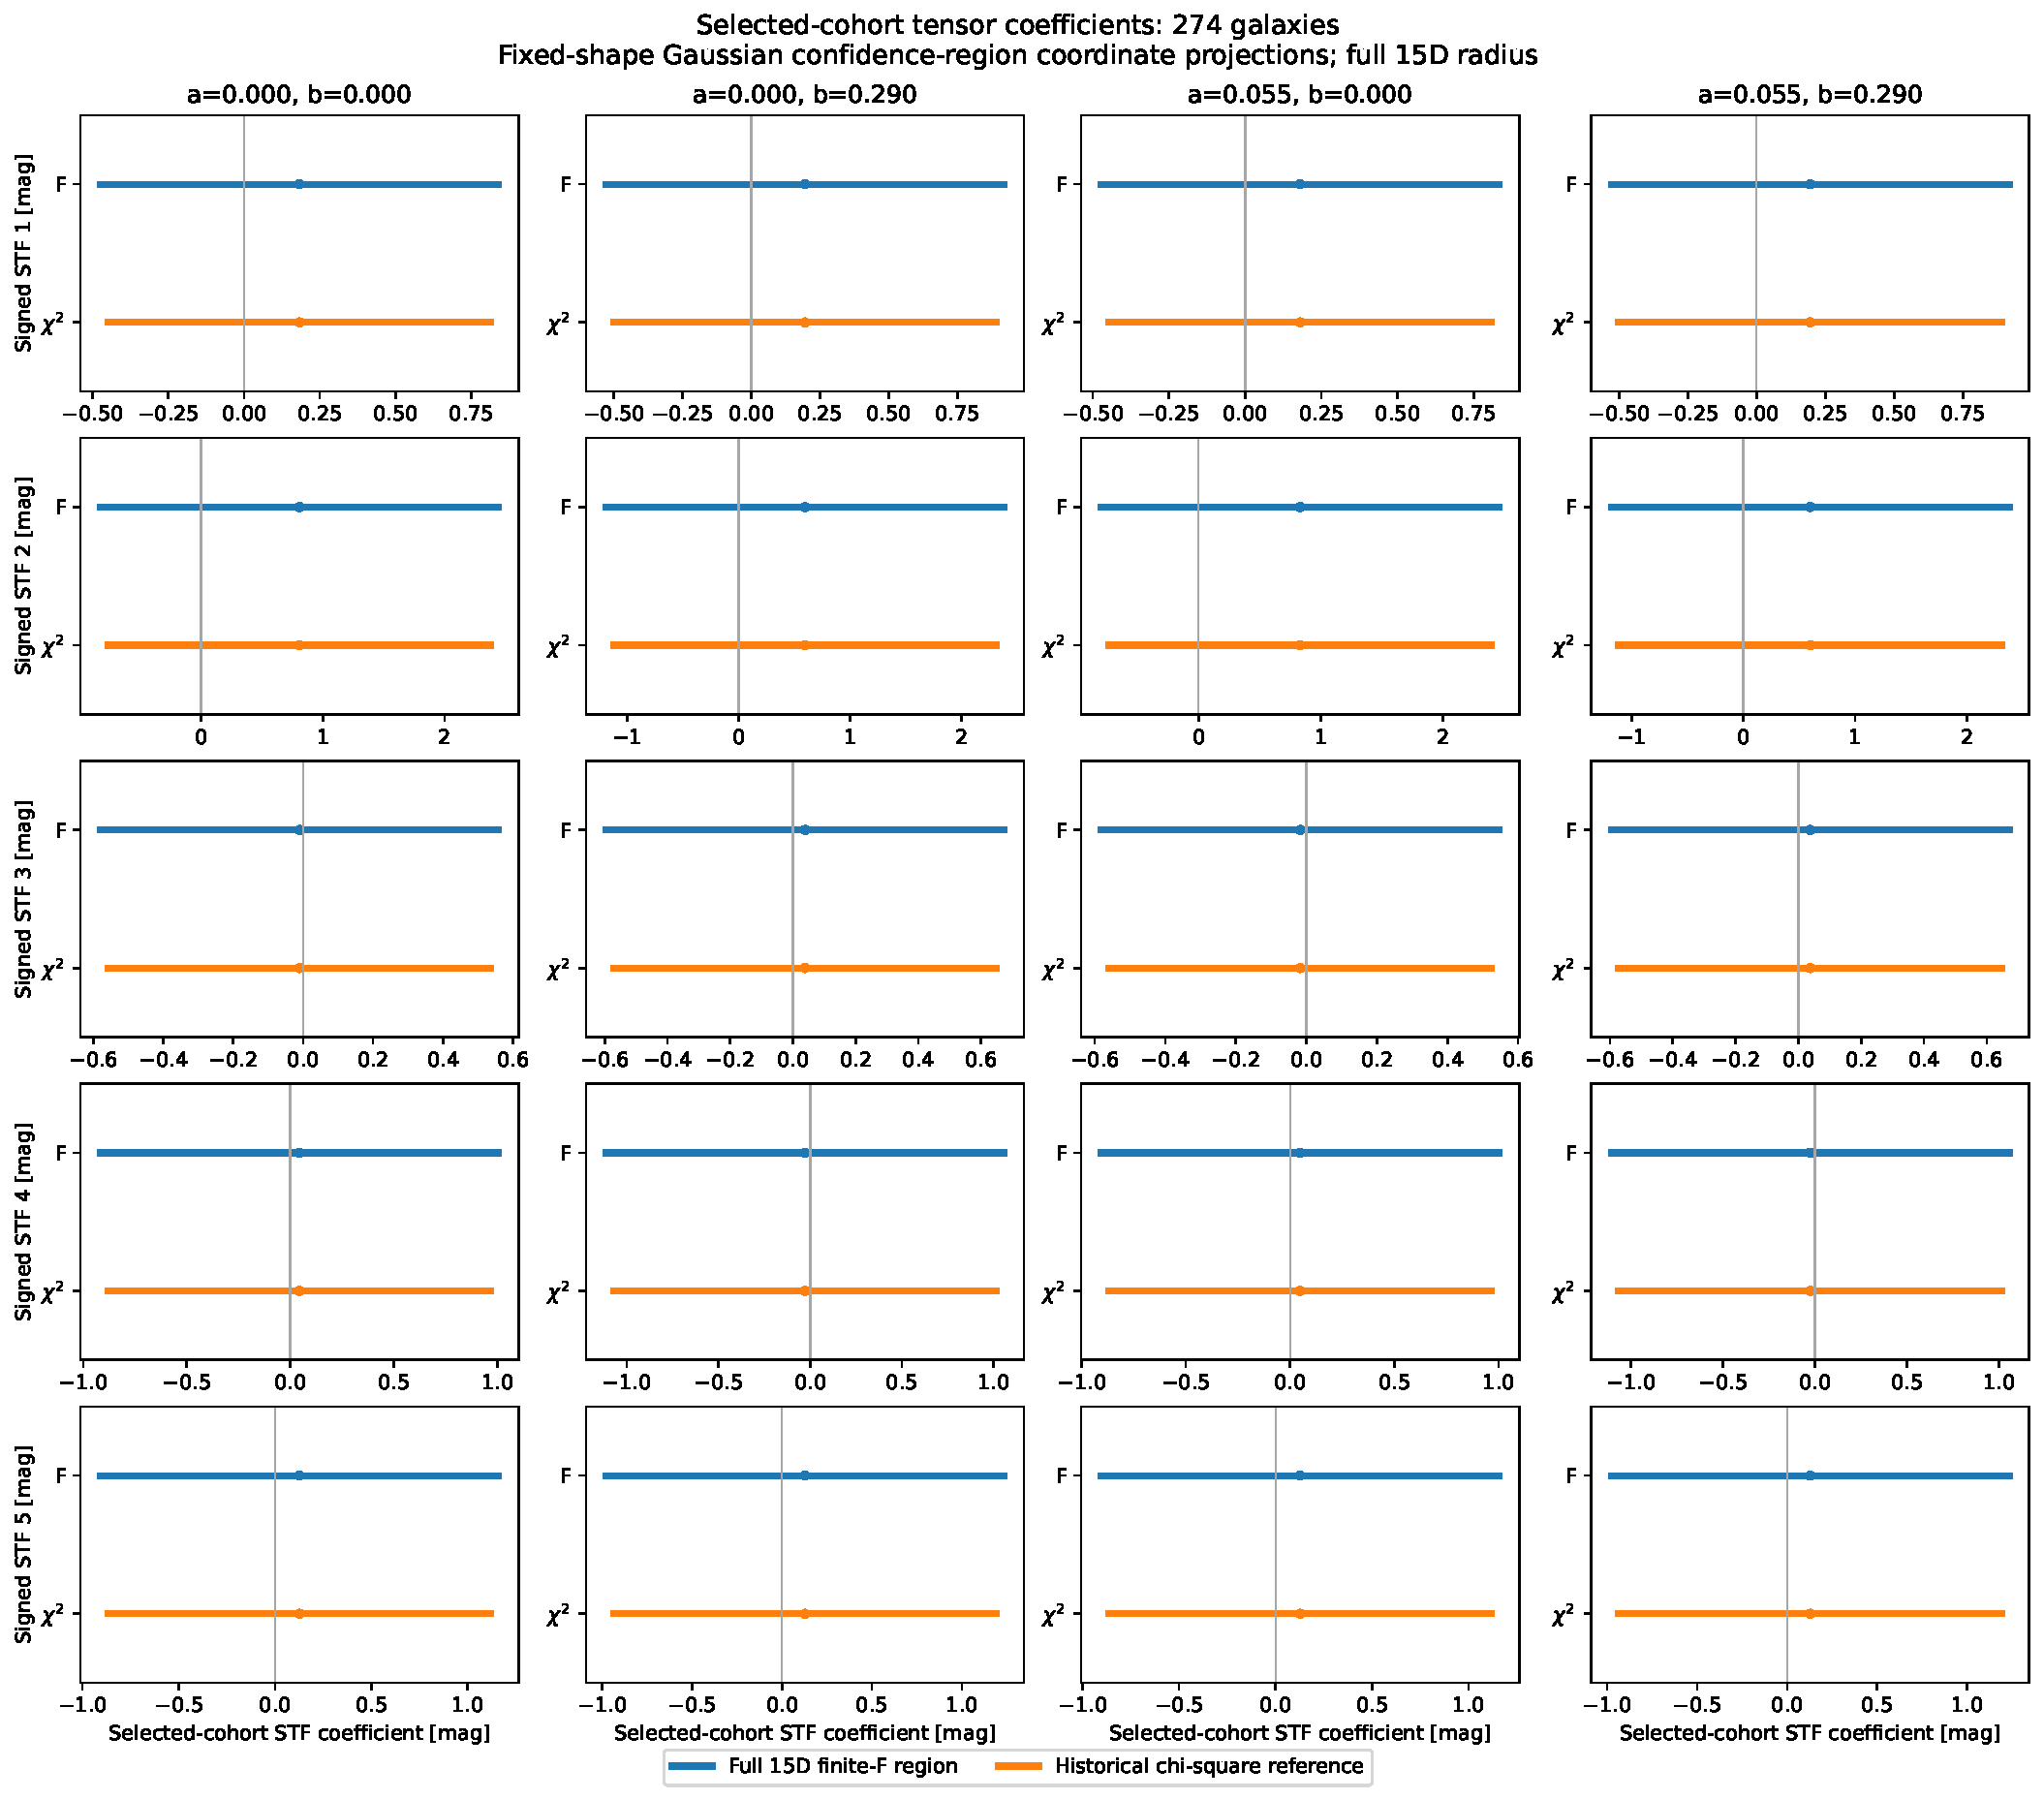
\includegraphics[width=.95\textwidth,height=.76\textheight,keepaspectratio]{figures/selected_tensor_law.pdf}
\caption{Five signed STF coordinates under four covariance shapes. The finite-$F$ intervals are coordinate projections of the full fifteen-parameter model-conditional 95\% region, with all nuisance parameters retained before projection. The historical chi-square intervals are fixed-Gaussian algebraic references, not exact finite-sample regions for an estimated scale. The plotted intervals do not replace the joint tensor covariance and do not give physical shear bounds.}
\label{fig:regions}
\end{figure}

The smallest predictive two-sided tail across all twenty entries is $0.0232647095087$. None crosses $0.0025$. This statement is compatible with poor predictive scores for some models: the two calculations answer different questions. The finite-$F$ check includes training-coefficient uncertainty, whereas the saved scoring rule below uses a plug-in prediction covariance. In addition, a lack of rejection at a conservative retrospective threshold does not demonstrate an adequate physical model.

\subsection{Model comparison changes with group covariance}

We compare three retained mean models on exactly the same rows and whole-group folds. Model A has the four baseline columns, the shared calibration dipole, and the three $K_i n_i$ columns; it has ten coefficients. Model B replaces the latter vector response with five STF columns and has twelve coefficients. Model C includes both responses and has fifteen coefficients, as in Eq.~\eqref{eq:design}. These are competing selected-window mean descriptions, not three identified cosmological geometries.

For each fold the retained score uses the normalized block-conditional Gaussian density with mean in Eq.~\eqref{eq:predictor} and covariance $\widehat\sigma^2_{{\rm ML},t}W_s$. Training-coefficient and scale uncertainty are omitted from this plug-in density. We preserve that procedure rather than retrospectively replacing its scores with a different predictive law. Scores are summed over the five held-out blocks; larger values indicate better prediction for this scoring procedure within one covariance scenario. They are not marginal likelihoods or Bayes factors.

\begin{table}[htb]
\caption{Summed joint held-out log densities on the same 274 responses. Every row uses the same folds. The scores are retrospective plug-in comparisons with training-parameter uncertainty omitted; they are separate from Eq.~\eqref{eq:predf}.}
\label{tab:comparison}
\begin{ruledtabular}
\begin{tabular}{rrrrr}
$a$ [mag]&$b$ [mag]&A: vector response&B: STF response&C: both\\
0&0&$-220.320018$&$-196.843320$&$-518.193732$\\
0&0.29&$-194.273316$&$-195.138036$&$-209.534052$\\
0.055&0&$-231.854820$&$-198.339595$&$-651.993130$\\
0.055&0.29&$-193.723069$&$-194.545441$&$-209.464523$
\end{tabular}
\end{ruledtabular}
\end{table}

The ordering reverses. Model B leads when the added group covariance is zero; model A leads narrowly when $b=0.29\,\mathrm{mag}$. Model C performs poorly, especially without the group term. Hence the retained evidence does not support a covariance-insensitive preference for one angular response. Figure~\ref{fig:models} shows the score dependence together with signed residual summaries. Small aggregated residual means do not remove this instability or certify the residual distribution.

There is also a directly interpretable domain failure. For PGC 9031, with $V_{\rm CMB}=317\,\kms$, the fitted vector contribution in model C corresponds to a flow fraction approximately $2.26$--$2.45$ across the covariance choices. A small-velocity interpretation of Eq.~\eqref{eq:kresponse} is invalid there. The coefficient can remain a term in a phenomenological regression, but interpreting it as a perturbative physical flow would exceed its approximation domain. Removing that object after inspecting the scores would define a new analysis.

An earlier seven-column Gaussian residual candidate on this cohort also failed an actual-data check: its retained discrepancy was $T=4.555321823822732$, with three simulated values at least as extreme among 4096 reference realizations, giving the recorded plus-one rank $4/4097=0.000976324139614352$. This is a failure of that specified working residual candidate. It is not a calibrated test of the later A/B/C alternatives, and repeated simulations from the old candidate cannot repair its observed discrepancy. We retain the failure because model criticism must remain attached to the model and source on which it occurred.

\begin{figure}[p]
\centering
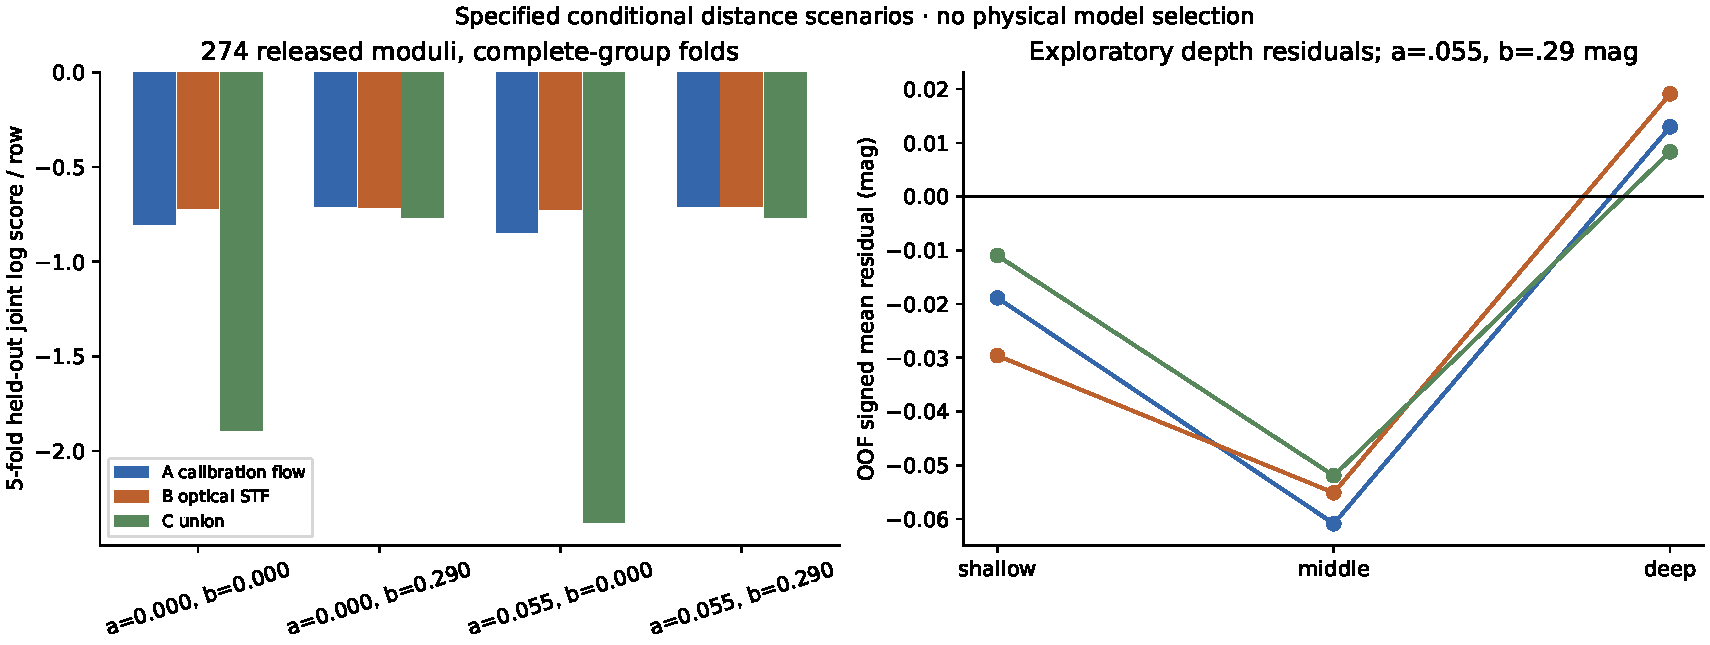
\includegraphics[width=.95\textwidth,height=.76\textheight,keepaspectratio]{figures/model_comparison.pdf}
\caption{Retained whole-group prediction scores and signed residual summaries for the three mean models on the same observed cohort. The ordering of vector and STF models changes with the declared group covariance. These plug-in scores do not include training-coefficient or scale uncertainty and are not the finite-$F$ diagnostics. The fitted angular terms remain selected-window responses.}
\label{fig:models}
\end{figure}

\subsection{Missing outcomes and the target-frame fraction}

For a fixed model and covariance choice, consider the event $|r_i|>t$ for the saved held-out signed residual $r_i$ in magnitudes. At $t=0.5\,\mathrm{mag}$, the count $m$ among the 274 observed objects ranges from 71 to 80 over the twelve retained cases. If the 354 missing event indicators are unrestricted, the exact attainable set of the uniform 628-target fraction is
\begin{equation}
 \mathcal J_m=\left\{\frac{m+k}{628}:k=0,1,\ldots,354\right\}.
 \label{eq:missingframe}
\end{equation}
Its smallest containing interval has width $354/628=0.5636942675$. The set itself is discrete. Reporting the hull does not make every intermediate fraction attainable by a deterministic completion.

We also vary a declared measure on the observed cohort. If its original uniform event mass is $e=m/274$ and the new density ratio lies in $[1/\Gamma,\Gamma]$ with mean one, then the sharp event-mass endpoints are
\begin{align}
 L_\Gamma(e)&=\max\{e/\Gamma,1-\Gamma(1-e)\},\nonumber\\
 U_\Gamma(e)&=\min\{\Gamma e,1-(1-e)/\Gamma\}.
 \label{eq:densitybounds}
\end{align}
The proof uses the constraints on the event and its complement, and constant within-class densities attain the endpoints. This is a normalized density-ratio class; two atomic density ratios may differ by $\Gamma^2$. It is not the different convention that bounds only the ratio between the largest and smallest weights.

Holding the observed target mass fixed at $274/628$, the completed set becomes
\begin{equation}
 \bigcup_{k=0}^{354}\left[
 \frac{274}{628}L_\Gamma(e)+\frac{k}{628},\;
 \frac{274}{628}U_\Gamma(e)+\frac{k}{628}\right].
 \label{eq:completedweighted}
\end{equation}
At $\Gamma=2$ and $t=0.5\,\mathrm{mag}$ its hull widths are $0.7333$--$0.7548$; at $\Gamma=4$ they are approximately $0.8909$. Figure~\ref{fig:selection} retains all model--shape cases rather than selecting a favourable curve. The availability fraction $274/628$ is not an estimated inclusion propensity for a larger population. These are mathematical sensitivity sets for the known finite target frame, not confidence intervals for a physical anisotropy fraction.

For signed means the limitation is stronger. Assigning an arbitrary common residual $R$ to all missing objects changes the target mean by $(354/628)R$. Its range is unbounded in that completion model. This statement requires no probabilistic imputation and does not assert a physically realizable range for a cosmological tensor. A physical support restriction, if justified separately, would change the identified set.

\begin{figure}[p]
\centering
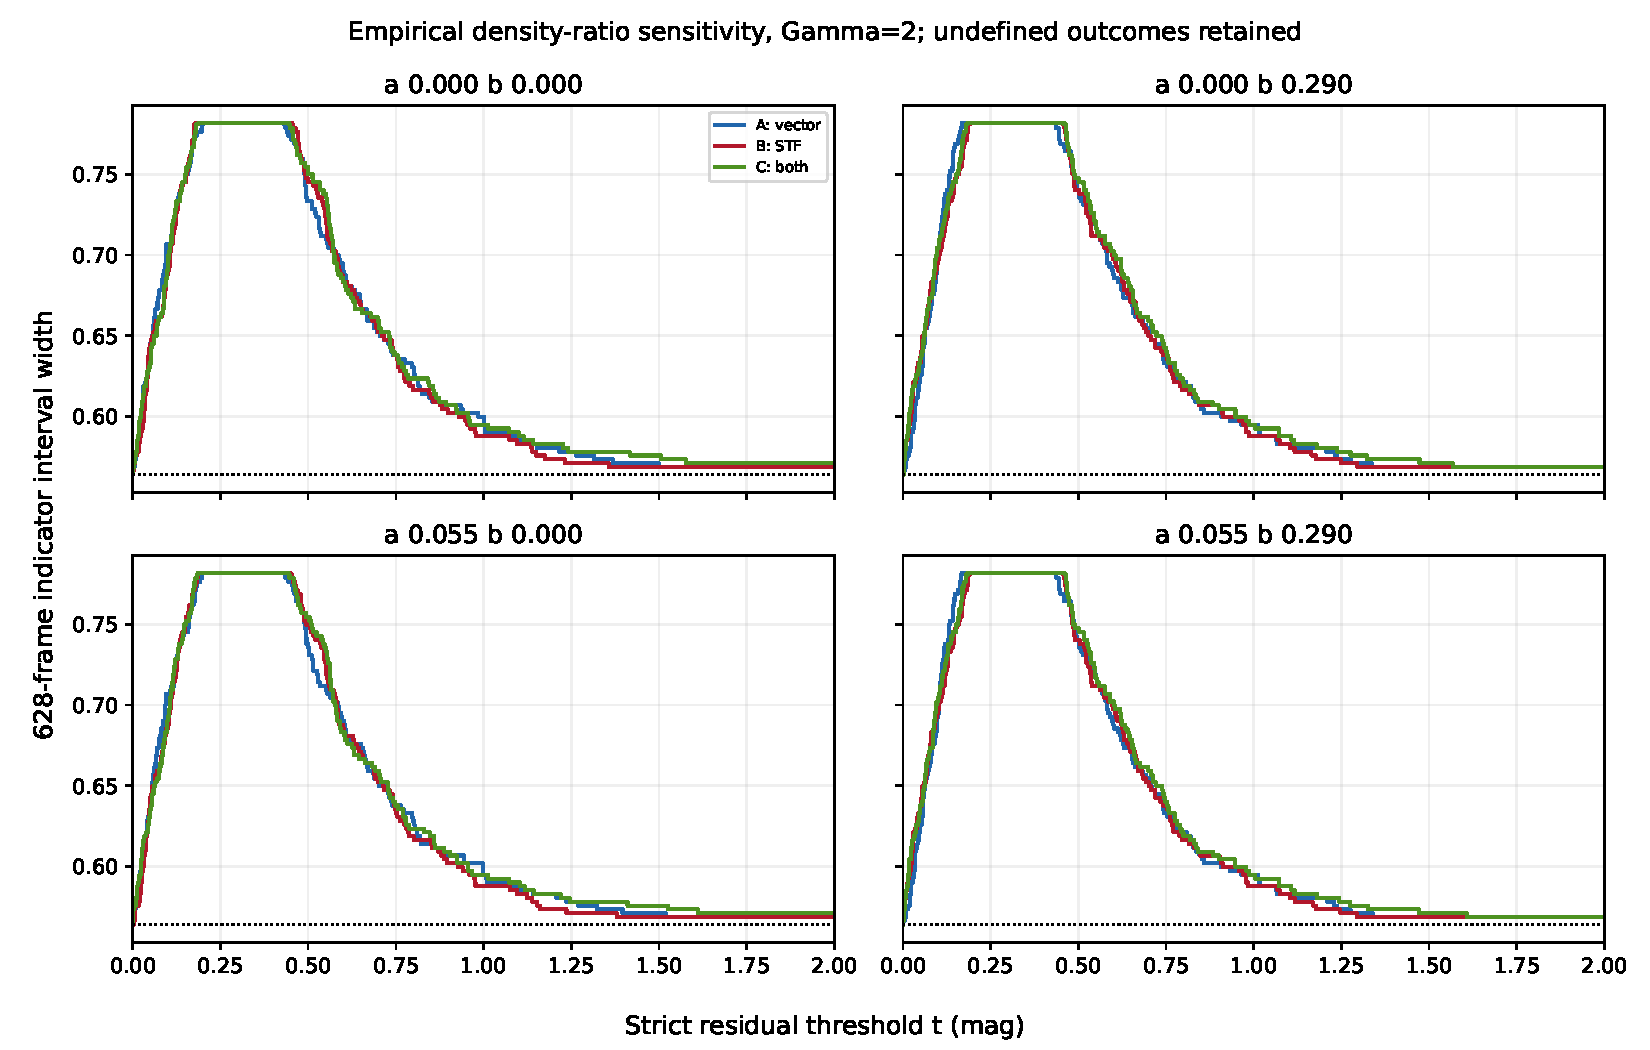
\includegraphics[width=.95\textwidth,height=.75\textheight,keepaspectratio]{figures/selection_bounds.pdf}
\caption{Finite-target sensitivity to weighting and missing event outcomes. The curves retain all twelve model--covariance cases at the declared density-ratio sensitivity level. The missing portion of the 628-target frame remains in every interval hull. At unit density ratio the exact attainable completion set is discrete, with hull width $354/628$. These curves do not estimate a parent selection law or a physical exceedance probability.}
\label{fig:selection}
\end{figure}

\subsection{Auxiliary balance cannot supply absent outcomes}

The retained auxiliary-total calculation provides a source-linked check of transport assumptions. Three cells of the 628-target frame contain no observed distances. Exact nonnegative balance over the full frame is therefore impossible: a positive target mass in any such cell cannot be generated from zero observed support. Deleting those cells defines a different 625-target frame. On this restricted frame, positive weights exist, range from $0.0021333333$ to $0.0064$, and have concentration effective sample size $1/\sum_i p_i^2=271.537086$.

This feasible balancing problem still leaves 351 outcomes missing within supported cells. Finer velocity balancing fails even with signed weights: an observed linear functional vanishes, whereas its target value is nonzero, corresponding to a $2547\,\kms$ discrepancy in the retained within-cell velocity total. Thus the problem is not solved by allowing negative weights or reporting a large concentration effective sample size. The weights constrain auxiliary totals, not the missing response values.

The same positive weights were applied jointly to each retained residual scalar, direction vector, and full STF residual tensor for every model--shape case. This preserves their common atomic dependence. It is a coherent change of finite measure, with no claim that balance proves missing-at-random sampling. In particular, separately choosing weights to improve each scalar summary would no longer describe one transported tensor law.

\section{Physical response and a separate coupled functional example}
\label{sec:coupled}

\subsection{Physical nonidentification within a declared domain}

Consider the explicit small-anisotropy optical-response scenario
\begin{equation}
 B=-kS+b_{\rm opt},\qquad k=\frac{5}{\ln10},\qquad
 S=\sigma_u/H_u,
 \label{eq:opticalresponse}
\end{equation}
where $B$ and $b_{\rm opt}$ are STF tensors in magnitudes and $S$ is a dimensionless physical shear ratio in a specified observer congruence. We restrict $S$ to a declared admissible domain $\mathcal D_S\subseteq\STF$, on which this optical approximation is intended to apply. For example, a small-anisotropy scenario may choose $\mathcal D_S=\{S:\|S\|_F\leq\epsilon\}$ for a specified small $\epsilon>0$; no measured value of $\epsilon$ is supplied here. The subscript distinguishes the optical bias tensor from the scalar group-covariance scale $b$ in Eq.~\eqref{eq:covariance}. The response coefficient $k$ carries the magnitude convention. The bias includes whatever calibration and optical-remainder contribution is admitted in this scenario. No measured bound on it is supplied.

For every $S'\in\mathcal D_S$, choosing
\begin{equation}
 b'_{\rm opt}=B+kS'
 \label{eq:biaswitness}
\end{equation}
leaves the observed $B$ unchanged. Within this response scenario, unrestricted optical bias therefore gives
\begin{equation}
 \mathcal I_S(B;\mathcal D_S)
 =\{S\in\mathcal D_S:\exists\,b_{\rm opt}\in\STF,\ B=-kS+b_{\rm opt}\}
 =\mathcal D_S.
 \label{eq:admissibleshear}
\end{equation}
The observation does not distinguish any two shear tensors in the declared domain. If $\mathcal D_S$ is the small norm ball above, this image is bounded. Only the formal affine extension $\mathcal D_S=\STF$ has an unbounded image and unbounded squared norm; that extension is not justified by a small-anisotropy premise. The normalized selected likelihood can still identify $\beta$ and bound its tensor projection, because the physical decomposition in Eq.~\eqref{eq:opticalresponse} is not part of that identified regression parameter. This is the relevant fibre obstruction.

The statement is conditional on both the specified response model and its admissible domain. It is not a measured bias, a universal impossibility theorem for shear observations, or a claim that every tensor in the formal affine extension satisfies a complete cosmological solution. Restricting the bias or supplying further physical response information can shrink the set within $\mathcal D_S$. Replacing $b_{\rm opt}$ by zero without evidence would instead choose a representative that may not even belong to that domain.

For example, a separately justified bound $\|b_{\rm opt}\|_F\leq\rho_B$ would give the finite algebraic outer set
\begin{equation}
 \mathcal S^{\rm out}_{\rho_B}
 =\bigcup_s\left\{-\frac{B}{k}+r:B\in\mathcal B_s,
                               \|r\|_F\leq\frac{\rho_B}{k}\right\}.
 \label{eq:boundedimage}
\end{equation}
The corresponding domain-restricted image within this scenario is $\mathcal D_S\cap\mathcal S^{\rm out}_{\rho_B}$. For a test tensor $U$, the support function of the unrestricted algebraic outer set is
\begin{equation}
 h_{\mathcal S^{\rm out}_{\rho_B}}(U)
 =\max_s\left[-\frac{U:\widehat B_s}{k}
 +\frac{\sqrt{c_{0.05}\,u^TC_{B,s}u}}{k}\right]
 +\frac{\rho_B\|U\|_F}{k},
 \label{eq:supportimage}
\end{equation}
where $u_a=U:E_a$. For a restricted $\mathcal D_S$, this is generally an upper bound on the support of the domain-intersected image, not its exact support. The formula exhibits exactly where a bias bound would enter; it does not estimate one or certify the domain of the optical approximation. A support function describes the closed convex hull of a set; retaining the union in Eq.~\eqref{eq:boundedimage} and its domain intersection preserves information that the outer support function alone may discard.

Even such a shear image would not determine Eq.~\eqref{eq:xc}. The vorticity, tilt, curvature, and reference-congruence relation would remain additional inputs. A finite optical STF estimate therefore cannot be substituted for the full signed physical departure. This is why the physical $x_C$, $Q_C$, eligible $F$, and $G_F$ have no numerical physical estimates here.

\subsection{A separate apparent Hubble-rate carrier}

The four-window example uses 35\,970 Cosmicflows-4 groups, with distances $d_i=10^{(\mu_i-25)/5}\,\mathrm{Mpc}$ and recession variable $u_i=cz_{{\rm CMB},i}$. Its retained mean model in window $j$ is
\begin{equation}
 u_i=d_i\left[H_j+D_j\cdot n_i+n_i^TT_jn_i\right]+\epsilon_i.
 \label{eq:apphubble}
\end{equation}
The apparent tensor $T_j$, vector $D_j$, and monopole $H_j$ have units of $\hunit$. They are not the magnitude tensor $B$ or the physical tensor $S$ in Eq.~\eqref{eq:opticalresponse}. No source-qualified response from this apparent rate carrier to physical shear is available. Its physical response and physical identified set remain unknown; the optical witness in Eq.~\eqref{eq:biaswitness} cannot be transferred to this carrier by changing the label.

The windows have centres $z_j=(0.025,0.040,0.060,0.080)$ and Gaussian width $0.012$. The retained working row variance is
\begin{equation}
 s_{u,i}^2=(250\,\kms)^2+
 \left[70\,\hunit\,\frac{\ln10}{5}d_i e_{\mu,i}\right]^2,
 \label{eq:ratevariance}
\end{equation}
with diagonal errors across groups in this working model. Its window weight is proportional to $\exp[-(z_i-z_j)^2/(2\,0.012^2)]/s_{u,i}^2$. The four nine-coordinate fits form one 36-coordinate vector. If $A_j$ is the retained linear fitting operator, the cross-window covariance is
\begin{equation}
 C_{jk}=A_j\diag(s_{u,i}^2)A_k^T.
 \label{eq:crosswindow}
\end{equation}
All windows reuse the same groups. Their statistical dependence is not optional.

For example, the first two fitted monopoles have correlation approximately $0.702$. Their difference has formal standard deviation $0.09610\,\hunit$ under this working law, whereas deleting their covariance would give $0.17590\,\hunit$. The latter calculation changes the uncertainty substantially without changing the point estimates. Neither number includes a released joint calibration or peculiar-velocity covariance that is absent from the working law.

The saved coefficients also permit residual inspection without a new fit. The weighted residual root-mean-square values at the four window centres are approximately $(1111.45,1584.61,2730.94,3990.87)\,\kms$. Weighted standardized centred second moments are $(1.37372,1.37384,1.32522,1.16254)$. These are diagnostics of the saved apparent coefficients on the original groups, not independent Gaussian draws or a calibrated goodness-of-fit test. Their nontrivial values remain visible beside the functional summaries.

\subsection{One finite measure, anchors, and floors}

The retained joint summary supplies a stipulated 36-dimensional Gaussian reference with the full covariance in Eq.~\eqref{eq:crosswindow}. A previously constructed deterministic quadrature uses 1024 scrambled Sobol points and their antithetic partners, giving 2048 coupled atoms with common weight $1/2048$. One atom contains all four windows and every coefficient. The stored scramble seed is 160916; no new points are drawn for this paper. Finite-measure masses below are exact sums on those retained atoms, not independent Monte Carlo probabilities or empirically calibrated physical posterior probabilities.

On the positive-$H_j$ branch, define the apparent quantities
\begin{equation}
 A_j=\frac{\|T_j\|_F}{H_j},\qquad
 v_{ja}=\frac{t_{ja}}{H_j},\qquad
 q^{\rm app}_j(B_*)=\frac{A_j}{B_*},\quad B_*>0.
 \label{eq:apparent}
\end{equation}
All five signed $v_{ja}$ values are retained. The scalar $A_j$ is one projection of their tensor state. The anchor $B_*$ is a declared dimensionless comparison scale, distinct from the observed magnitude tensor $B$. It is not a measured physical shear bound, and $q_j^{\rm app}$ is not $Q_C$.

\begin{table}[htb]
\caption{Apparent tensor-to-monopole ratios from one coupled reference measure. The quantiles refer to its 2048 retained atoms. The last two columns use previously fitted coefficients under the baseline angular weight and the alternative factor $1+0.6n_z$; they are same-source sensitivity calculations without an alternative uncertainty law.}
\label{tab:apparent}
\begin{ruledtabular}
\begin{tabular}{rrrrr}
$z_j$&Median $A_j$&5--95\% finite-measure range&Baseline fit $A_j$&North-weighted fit $A_j$\\
0.025&0.02987439&[0.02320629, 0.03705731]&0.02882516&0.02768206\\
0.040&0.04299340&[0.03546864, 0.05056393]&0.04216629&0.04592671\\
0.060&0.05126981&[0.04329702, 0.05979327]&0.05034101&0.05053997\\
0.080&0.03111974&[0.02080593, 0.04326388]&0.02695545&0.02241775
\end{tabular}
\end{ruledtabular}
\end{table}

For the reference window $j=0$, the paired apparent contrast is
\begin{equation}
 g_j^{\rm app}(B_*,\delta)
 =\frac{\max(A_j/B_*,\delta)}{\max(A_0/B_*,\delta)}
 =\frac{\max(A_j,B_*\delta)}{\max(A_0,B_*\delta)}.
 \label{eq:flooridentity}
\end{equation}
Thus the entire paired array depends on the product $B_*\delta$. When the floor is inactive, the common anchor cancels; with fixed $\delta$, changing the anchor changes the effective floor. This exact identity explains an otherwise misleading impression of anchor robustness.

At effective floor $0.005$, the median ratio for the $z=0.060$ window relative to $z=0.025$ is $1.718693$. At effective floor $0.05$, it is $1.025396$. At $0.075$, every retained paired ratio equals one and the strict mass of $g_j^{\rm app}>1$ is zero. The tensor coefficients have not become equal. The chosen floor has erased their distinction.

The joint event $\max_j A_j>0.05$ has retained mass $1235/2048=0.60302734375$. It is computed on one coupled atom at a time, not by multiplying four marginal probabilities. The normalized density-ratio class in Eq.~\eqref{eq:densitybounds} changes this event mass to the interval $[0.301513671875,0.801513671875]$ at $\Gamma=2$. This is a sensitivity envelope for a finite reference measure, not a physical credible interval. Figure~\ref{fig:functionals} displays the anchor, floor, weighting, and window dependence together.

\begin{figure}[p]
\centering
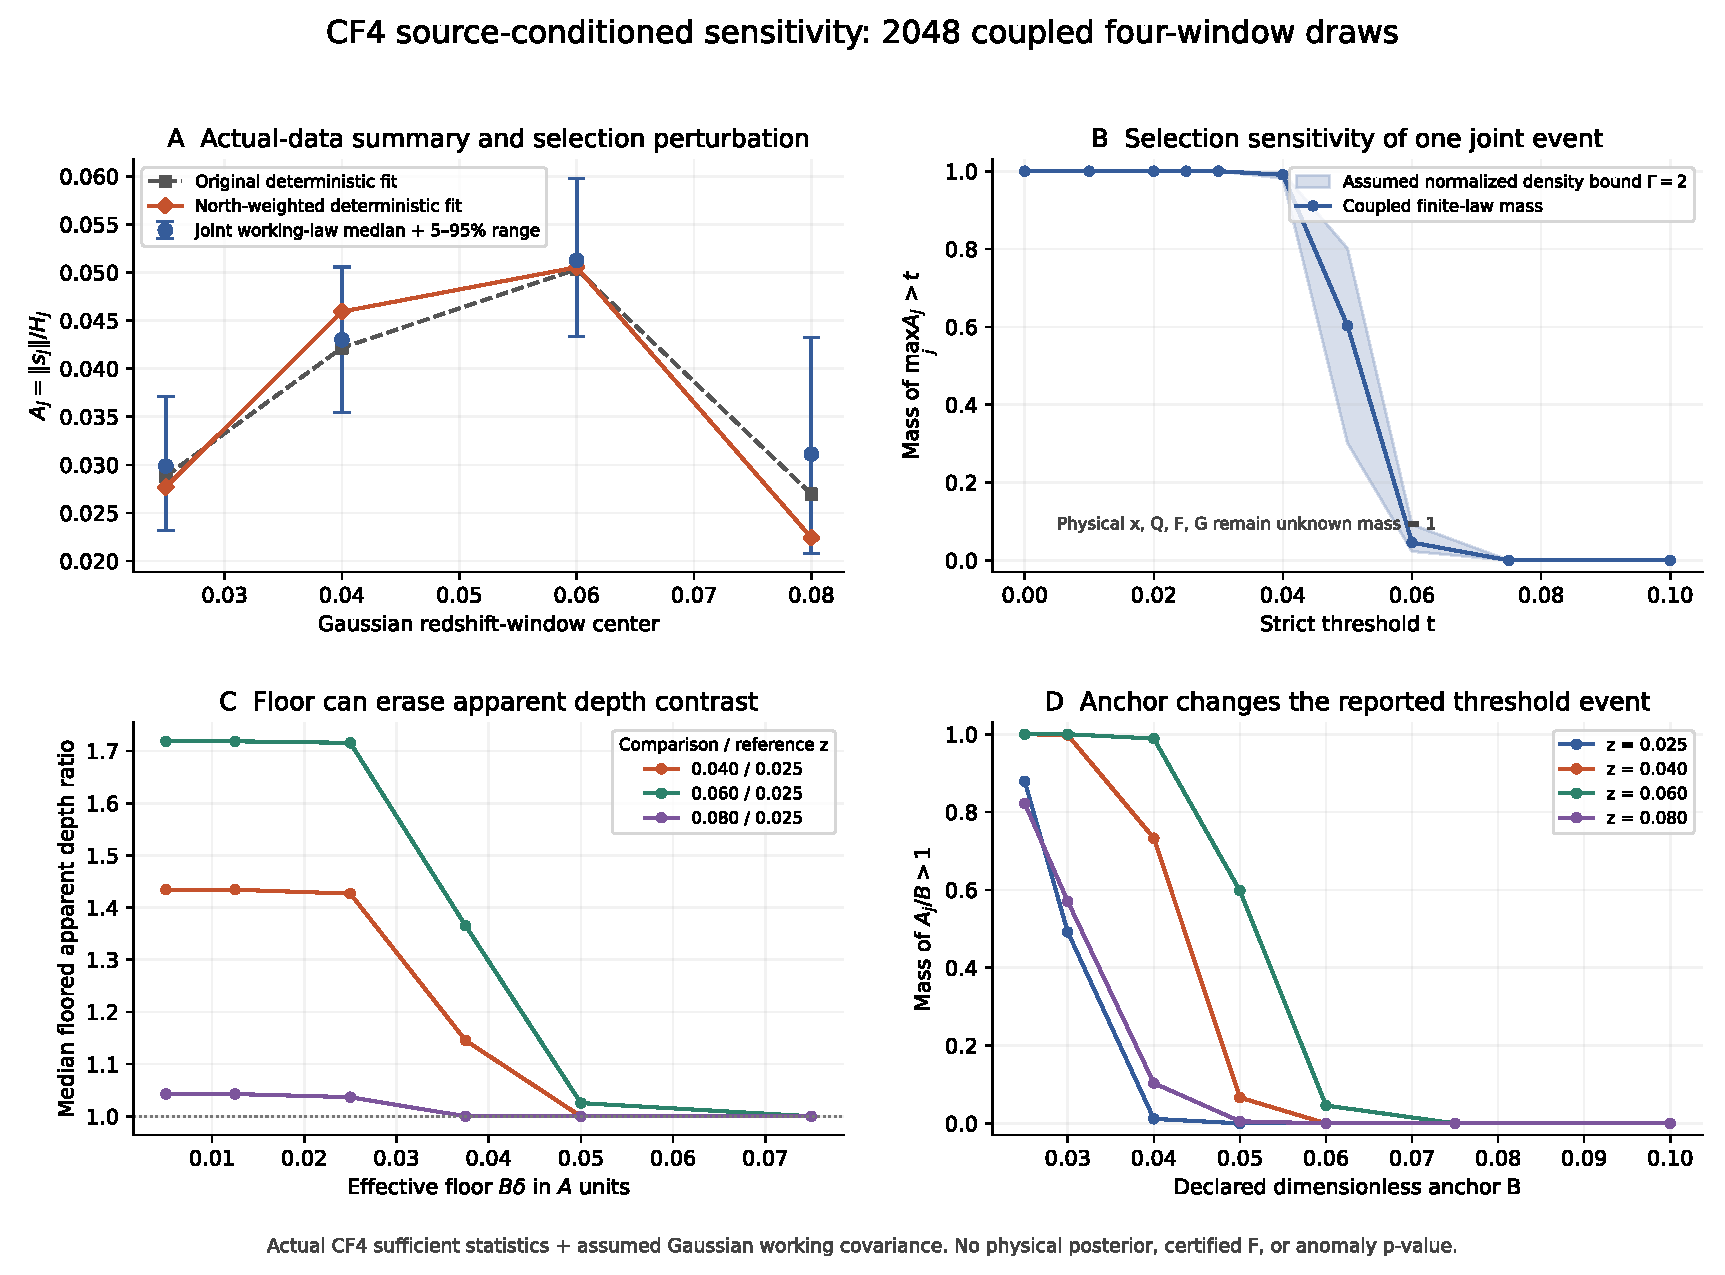
\includegraphics[width=.95\textwidth,height=.75\textheight,keepaspectratio]{figures/coupled_functionals.pdf}
\caption{Functional sensitivity of the separate four-window apparent Hubble-rate carrier. The blue quadrature summary in panel A and the summaries in panels B--D use the same retained 2048 coupled quadrature atoms and full cross-window covariance. Panel A also shows the deterministic baseline and north-weighted fits as estimator comparisons. The north-weighted covariance is unavailable, so these fits do not supply an alternative 2048-atom law or an uncertainty law for their difference. The apparent tensor norm, declared anchor, positive floor, and normalized density-ratio envelope have distinct roles. Finite-measure quantiles and masses are conditional on the stated reference construction; they do not constitute physical $Q_C$, $F$, $\Pi$, or $G_F$ measurements.}
\label{fig:functionals}
\end{figure}

Changing actual angular weights provides a different sensitivity check. The north-weighted apparent ratio differs from the baseline by approximately $-3.966\%$, $+8.918\%$, $+0.395\%$, and $-16.834\%$ across the four windows. Its covariance was not retained, so no new distribution is assigned to these shifts. Likewise, a stored method-deletion result supplies the norm of a tensor change rather than its direction. We use triangle-inequality outer intervals, not an invented deleted tensor. For deletion of the fundamental-plane family in the highest-redshift window, the retained interval for $A_j$ is $[0,0.06357699208]$. These calculations show source and estimator sensitivity on one catalogue.

\subsection{Unknown mass is not a zero-valued functional}

For a normalized finite measure with atom weights $p_i$, let $K$ be the indices where a functional is defined and known and let $U$ be the remaining indices. If $a_t=\sum_{i\in K}p_i\ind\{q_i>t\}$ and $u=\sum_{i\in U}p_i$, unrestricted completion of the unknown event indicators gives
\begin{equation}
 a_t\leq\Pi_{\mu,q}(t)\leq a_t+u.
 \label{eq:unknownmass}
\end{equation}
The two endpoints are attainable for unconstrained binary completions. Functional range restrictions can make them conservative rather than sharp; an eligible $F\leq1$, for example, cannot exceed one. A domain failure need not admit any physical completion at all. We therefore record domain failure separately from a defined but unmeasured value.

The present apparent carrier does not qualify physical $x_C$, $Q_C$, $F$, or $G_F$ on any atom. Its physical unknown mass is one. The generic interval $[0,1]$ records absence of a qualified physical event law, not a measured broad posterior and not a claim of physically sharp attainability at every threshold. Renormalizing only known values would instead condition on being known, changing the question. Ordered exceedance thresholds must also share one completed value per atom, so arbitrary independent choices from their marginal intervals need not define a possible exceedance curve.

\section{Discussion and conclusions}
\label{sec:discussion}

The selected-distance calculation identifies a statistical coefficient under an explicit law. It provides a normalized real-row likelihood, a finite-$F$ confidence region for the joint fifteen-coordinate mean, and tensor projections that preserve nuisance uncertainty. The main limitation is not failure to propagate that uncertainty. It is the additional information needed to interpret the coefficient physically and to transport it beyond the released cohort.

The model comparison makes that limitation measurable. The vector and STF models exchange predictive ordering when the declared group covariance changes. A low-velocity object violates the perturbative interpretation of the vector response, and an earlier residual candidate fails an actual-data check. These are substantive results of model criticism. They cannot be replaced by the statement that no later fold diagnostic crosses a conservative reference threshold. The later finite-$F$ calculation changes the treatment of training uncertainty and qualifies a conditional coefficient region; it does not retrospectively erase the earlier failure or validate the parent sampling law.

Selection produces another obstruction. The exact finite-completion set retains every missing event indicator, giving a hull at least $0.56369$ wide for the 628-target fraction. Auxiliary balance identifies useful feasible weights only after the target is changed, and even then it leaves missing outcomes unresolved. This prevents the observed fraction, a balanced fraction, and a parent-population probability from being used interchangeably. Each is an estimand under different information and assumptions.

The optical-response example separates statistical from physical identification particularly clearly. Under an unrestricted additive STF bias, the identified shear image equals its declared admissible domain $\mathcal D_S$. The selected likelihood cannot distinguish its members. A bounded small-anisotropy domain therefore gives a bounded image, while unboundedness belongs only to the formal affine extension $\mathcal D_S=\STF$. A justified response-bias bound would enter the algebraic outer-support formula explicitly and could further restrict the domain-intersected image. It would still leave the other signed sectors of $x_C$ and the common reference frame to be supplied. The corresponding physical response for the separate apparent Hubble-rate carrier is presently unknown; neither this optical identified-set formula nor its formal unbounded extension is transferred between their different units.

This distinction also limits the meaning of the functional bundle. Full tensors, signs, cross blocks, and domain states carry information that scalar normalizations can remove. A reference anchor defines a comparison scale. A positive floor defines how small values are treated. Neither is inferred merely because its value makes a plot stable. In the retained four-window example, changing the effective floor moves a median ratio from $1.718693$ to $1.025396$ and eventually makes every ratio one. The observable carrier is unchanged throughout.

The theoretical statements used here are elementary or standard specializations: fibre identification, Gaussian regression pivots, projection of a common confidence event, union coverage under a true member of a fixed family, and bounded-density event envelopes. We make no claim of priority for those results. The methods contribution is their source-linked application to real selected tensor data, including the failure and nonidentification cases. Ordinary pushforward remains a valid operation once a law and a defined functional are supplied. The present analysis determines where those inputs are available and where they are not.

Further physical inference would need source-matched response calibration, justified covariance and selection laws, and compatible frame and normalization information. A physical family comparison would additionally require family-specific predictions and null competition; a tensor amplitude or morphological match alone cannot identify a homogeneous cosmological geometry. These missing ingredients do not prevent the selected likelihood and sensitivity results from being reported. They determine their scope.

\section*{Data and computational provenance}

The observational inputs are the published Cosmicflows-4 products, the retained linewidth-target join, and identifier-matched directions from CDS/HyperLEDA. The two analysed source populations are described separately in Secs.~\ref{sec:likelihood} and \ref{sec:coupled}. The accompanying source map links each numerical table and figure to the retained results, row identities, response conventions, and scoped checks. It preserves the full coefficient and cross-window covariances rather than reconstructing them from marginal intervals. The manuscript consumes these results without new fitting or drawing. Figure preparation changes publication labels or file format while retaining the numerical content. No cross-survey likelihood multiplication or physical response imputation is used.

\appendix
\section{Information and domain statements}
\label{app:fibres}

The identification criterion in Eq.~\eqref{eq:fibre} follows in both directions. If $h=\widetilde h\circ\mathcal O$ for a function on observation laws, then two states with the same law have the same target. Conversely, if $h$ is constant on each fibre, define $\widetilde h(o)$ as that common value. It is well defined on the image of $\mathcal O$. The same argument applies to a deterministic compression $T$: a target can be recovered from $T$ if and only if it is constant on each fibre of $T$. A norm-only representation of the STF tensor fails that test for determinant, eigenvalue shape, and oriented directional contractions.

For a partially defined target one must retain the domain statement as well. A fibre entirely inside $\mathcal D_h$ may have a singleton, bounded, or unbounded image. A fibre intersecting both $\mathcal D_h$ and its complement has an additional unresolved domain status. A fibre disjoint from $\mathcal D_h$ does not yield a zero target. These distinctions survive confidence-set propagation. In particular, a singular normalization should not be replaced by a numerical floor unless the target is explicitly changed to the floored functional.

Equation~\eqref{eq:coverageimage} holds for any collection of deterministic functions defined at the true state, because the same membership event implies every image membership. The coverage level belongs to that original joint event. This argument does not authorize selecting the confidence procedure after inspecting its success, inferring a probability measure inside the set, or treating a physical response relation as known when it was omitted from the construction.

\section{Gaussian pivots and nuisance projection}
\label{app:pivot}

Whiten the selected model by $V_s^{-1/2}$. The whitened residual vector is an isotropic Gaussian vector, and its projections onto the column space of $V_s^{-1/2}X$ and the orthogonal complement are independent. Their dimensions are $p$ and $n-p$. Thus
\begin{equation}
 \frac{(\widehat\beta_s-\beta)^TG_s(\widehat\beta_s-\beta)}{\sigma^2}
 \sim\chi^2_p,\qquad \frac{q_s}{\sigma^2}\sim\chi^2_{n-p},
\end{equation}
independently. Their scaled ratio proves Eq.~\eqref{eq:fpivot}. Since $C_{{\rm ML},s}^{-1}=(n/q_s)G_s$, multiplication by $np/(n-p)$ gives Eq.~\eqref{eq:finitef}. Using a chi-square radius with this estimated scale would skip the denominator uncertainty.

For a full ellipsoid $\{\Delta:\Delta^TC^{-1}\Delta\leq c\}$, minimizing the quadratic over nuisance coordinates at fixed $P_B\Delta$ gives $(P_B\Delta)^T(P_BCP_B^T)^{-1}(P_B\Delta)$. This proves Eq.~\eqref{eq:tensorregion}. It is a projection result. By contrast, fixing the nuisance coordinates at zero would use the relevant precision block and generally a narrower section. Cross blocks affect the original joint geometry even when its projection can be written using the covariance submatrix.

For the prediction pivot, decompose the validation error as
\begin{equation}
 e_v=\left(Y_v-R_sY_t-D_s\beta\right)
                         -D_s(\widehat\beta_{t,s}-\beta).
\end{equation}
The first term is a Gaussian innovation with covariance $\sigma^2W_s$, independent of the training outcomes. The second is Gaussian with covariance $\sigma^2D_sG_{t,s}^{-1}D_s^T$. Both are independent of the training residual quadratic: for the second term this follows from the training Gaussian projection. Hence $e_v^TM_s^{-1}e_v/\sigma^2\sim\chi^2_m$ independently of $q_{t,s}/\sigma^2\sim\chi^2_{n_t-p}$, proving Eq.~\eqref{eq:predf}. The proof requires positive-definite shapes, full training rank, a correct common mean, and the Gaussian law. It neither removes cross-validation dependence nor gives a law conditional on fixed realized training outcomes.

\section{Event completion and density-ratio endpoints}
\label{app:completion}

For a binary event of reference mass $e$, write $q$ for its mass after reweighting. Bounding the density on both the event and its complement gives
\begin{equation}
 \frac e\Gamma\leq q\leq\Gamma e,\qquad
 \frac{1-e}{\Gamma}\leq1-q\leq\Gamma(1-e).
\end{equation}
Their intersection is Eq.~\eqref{eq:densitybounds}. For $0<e<1$, choose densities $q/e$ on the event and $(1-q)/(1-e)$ on its complement. They are feasible at both endpoints. The cases $e=0$ and $e=1$ are immediate. This proves sharpness within the specified density class, not within an unmeasured physical selection process.

For the finite target frame, exactly $k$ of the 354 missing indicators can be set to one for each integer $0\leq k\leq354$. This establishes Eq.~\eqref{eq:missingframe} and, after observed-cohort reweighting, Eq.~\eqref{eq:completedweighted}. The interval hull is an outer representation of that finite union. For an arbitrary partially known weighted event, setting every unknown indicator to zero or one gives Eq.~\eqref{eq:unknownmass}; extra domain or range constraints can remove those extremizers.

At multiple thresholds $t_1<\cdots<t_m$, one scalar value has a nonincreasing exceedance-indicator vector. Therefore a common completion gives a weighted sum of threshold-prefix vectors. The product of separate pointwise intervals may include nonmonotone or otherwise unattainable curves. Likewise, separate weight choices that attain endpoints for different tensor functionals need not be one common measure. Retaining atom identity and applying the same weights is what makes the coupled calculation in Sec.~\ref{sec:coupled} a joint functional analysis.

\bibliographystyle{apsrev4-2}
\bibliography{references}
\end{document}
